\documentclass[conference,letterpaper]{IEEEtran}
\usepackage[utf8]{inputenc}
\usepackage[T1]{fontenc}
\usepackage[spanish,es-nodecimaldot]{babel}
\addto\captionsspanish{\renewcommand{\tablename}{Tabla}}
\renewcommand{\IEEEkeywordsname}{Palabras clave}
\usepackage{amsmath,amssymb,graphicx,booktabs,tikz}
\usepackage[hidelinks]{hyperref}
\newcommand{\doi}[1]{\href{https://doi.org/#1}{\nolinkurl{#1}}}
\graphicspath{{../figuras/}{figuras/}}
\title{Síntesis cinemática parcial de un mecanismo de exoesqueleto de dedo mediante Evolución Diferencial y Algoritmo Genético}
% La versión de evaluación define \versionciega antes de leer este archivo.
\ifdefined\versionciega
  \author{}
\else
  \author{
\IEEEauthorblockN{Adriana Elorza-Ramos\IEEEauthorrefmark{2}, Pavel Palma-Nicolás\IEEEauthorrefmark{1},\\
Manuel Arias-Montiel\IEEEauthorrefmark{1} y Esther Lugo-González\IEEEauthorrefmark{1}}
\IEEEauthorblockA{\IEEEauthorrefmark{1}Instituto de Electrónica y Mecatrónica\\
\IEEEauthorrefmark{2}División de Estudios de Posgrado\\
Universidad Tecnológica de la Mixteca, Huajuapan de León, Oaxaca, México\\
\texttt{\{eora010314,panp000112\}@gs.utm.mx}, \texttt{\{mam,elugog\}@mixteco.utm.mx}\\
\footnotesize ORCID: Adriana \href{https://orcid.org/0009-0008-8398-3191}{0009-0008-8398-3191};
Pavel \href{https://orcid.org/0009-0005-9704-9867}{0009-0005-9704-9867}\\
\footnotesize Manuel \href{https://orcid.org/0000-0003-4534-9401}{0000-0003-4534-9401};
Esther \href{https://orcid.org/0000-0002-7374-3425}{0000-0002-7374-3425}}
}

\fi
\begin{document}
\maketitle
\begin{abstract}
Este trabajo utiliza dos técnicas de optimización, la Evolución Diferencial (ED) y el Algoritmo Genético (AG), ambas implementadas en Python, para obtener la síntesis dimensional parcial de un mecanismo de exoesqueleto de dedo orientado a reproducir una pinza fina, ajustando el movimiento hasta la falange medial y la posición de su extremo, la articulación interfalángica distal (IFD). El problema se formula con 16 parámetros de diseño y una función objetivo de seguimiento angular respecto a una referencia de 120 muestras, obtenida de la base de datos \cite{r1}. Se añaden penalizaciones para mantener el cierre de los mecanismos, la separación respecto al dedo, la ubicación dorsal y una altura y transmisión adecuadas. La comparación utiliza los mismos límites, 20 semillas y 4096 evaluaciones por ejecución. Las soluciones seleccionadas alcanzan errores globales de posición de 0.298 mm para ED y 0.198 mm para AG. La ED produce un mecanismo más compacto según la suma de longitudes estructurales: 328.29 mm frente a 353.36 mm del AG. El AG obtiene menor error en ambos puntos: 0.169 mm en IFP y 0.222 mm en IFD, frente a 0.216 y 0.361 mm de ED. Por su menor tamaño, se elige la solución ED para construir el ensamble en SolidWorks y comprobar su movimiento. Sus trayectorias presentan errores respecto al modelo cinemático de 0.106 mm en IFP y 0.112 mm en IFD. Los resultados muestran un compromiso entre seguimiento y compacidad.
\end{abstract}
\begin{IEEEkeywords}
evolución diferencial, algoritmo genético, síntesis dimensional, exoesqueleto de mano, optimización dimensional, cadena de mecanismos.
\end{IEEEkeywords}

\section{Introducción}
Los exoesqueletos de mano son dispositivos robóticos de asistencia y rehabilitación cuya función es acompañar o ayudar a recuperar el movimiento de los dedos \cite{r2}. Para que la asistencia resulte cómoda y segura, el mecanismo debe reproducir con fidelidad las trayectorias articulares naturales del dedo a lo largo de todo el rango de flexión previsto. Las diferencias entre el movimiento del dedo y el dispositivo pueden generar fuerzas de reacción no deseadas en las articulaciones y afectar la comodidad del usuario \cite{r3}. Lograr ese seguimiento depende en gran medida de elegir correctamente las longitudes de los eslabones del mecanismo, un problema que se conoce como síntesis dimensional \cite{r4}.

La síntesis dimensional para generación de trayectoria es un problema de optimización difícil. El espacio de soluciones contiene amplias regiones en las que el mecanismo simplemente no ensambla o invierte su movimiento, y la relación entre las longitudes de los eslabones y la curva que describe el mecanismo es no lineal y presenta muchos óptimos locales. Por ello se emplean metaheurísticas poblacionales como la Evolución Diferencial (ED) y los Algoritmos Genéticos (AG), capaces de recorrer el espacio de búsqueda sin necesitar información de derivadas \cite{r4,r5}.

Aunque ambas técnicas de optimización se usan ampliamente, cuál de las dos resulta más eficaz depende de la naturaleza del problema, de cómo se representan las variables y del ajuste de los hiperparámetros \cite{r6,r7}. La elección entre uno u otro rara vez es evidente y casi siempre requiere ponerlos a prueba sobre el caso concreto que se quiere resolver.

La síntesis dimensional de eslabonamientos para generación de trayectoria se ha abordado históricamente con métodos analíticos y, más recientemente, con metaheurísticas, que permiten explorar funciones no convexas sin calcular sus derivadas \cite{r4,r5}. Los mecanismos de cuatro barras son un bloque de construcción recurrente en síntesis de trayectoria, por su simplicidad y su capacidad de aproximar curvas de acoplador con pocos parámetros \cite{r4,r5}. En exoesqueletos de dedo también se han estudiado cadenas de seis barras, como el mecanismo Stephenson-II \cite{r8}. Cuando se encadenan varias etapas de cuatro y cinco barras, el número de variables crece y aparecen distintas soluciones locales. Una modificación de longitud afecta no solo a la trayectoria de una etapa, sino también al movimiento que se transmite a la siguiente; por ello se estudia el conjunto de eslabones y no cada etapa por separado.

En el ámbito de los exoesqueletos de mano se ha empleado optimización basada en enjambres para ajustar las dimensiones de mecanismos que reproducen la flexión de los dedos \cite{r8}. La comparación directa entre familias de algoritmos también ha sido estudiada \cite{r6,r7}. Tanto ED como un AG de codificación real pueden trabajar con variables continuas. Su resultado depende de los operadores y de los parámetros elegidos, por lo que sigue siendo necesario estudiar su comportamiento sobre el mecanismo concreto \cite{r9,r10}.

Para comparar ED y AG, se mantienen la misma función objetivo, los mismos límites de diseño y el mismo número de evaluaciones \cite{r6,r17}. En cada par de ejecuciones se utiliza además una población inicial idéntica. Así, ambos métodos prueban la misma cantidad de diseños; igualar solo las generaciones no garantiza esa condición. La comparación considera el error de seguimiento y la suma de longitudes para elegir una solución adecuada para la fabricación.

Para que la comparación sea reproducible, se optimiza una versión parcial del mecanismo, que reproduce el movimiento hasta la falange medial. Este caso es más pequeño que el modelo completo de tres falanges, pero conserva las dificultades esenciales del problema: el acoplamiento entre etapas y las restricciones de ensamble y espacio sobre el dedo. Esto permite estudiar el efecto del algoritmo de optimización sin la complejidad añadida de la etapa distal. Además, se construye en SolidWorks el mecanismo con las dimensiones optimizadas por ED y se comprueban sus trayectorias.

\subsection{Contribuciones}
Las contribuciones de este artículo son: (i) una formulación del problema de síntesis dimensional parcial con 16 parámetros y restricciones geométricas; (ii) una comparación de ED y AG con el mismo presupuesto y varias semillas, considerando error y tamaño; y (iii) la comparación entre el modelo cinemático y el estudio de movimiento del mecanismo optimizado en SolidWorks.

\section{Modelo cinemático del exoesqueleto}
 La Fig.~\ref{fig:dedo} muestra el diseño de partida; las dimensiones resultantes de la optimización se presentan más adelante. El dispositivo reproduce la flexión del dedo mediante una cadena de etapas acopladas accionadas por una única manivela de entrada $L_1$. La primera etapa combina un mecanismo de cinco barras ($L_1$, $L_2$, $L_3$, $L_4$ y la bancada $B_1$) y uno de cuatro barras ($L_4$, $L_5$, el soporte equivalente y la bancada $B_2$). Los desplazamientos $h_{sp}$ y $d_{sp}$ forman un soporte rígido cuya distancia entre centros es $\sqrt{h_{sp}^2+d_{sp}^2}$. Esta etapa lleva el movimiento desde la articulación metacarpofalángica (MCF) a la falange proximal.

La siguiente etapa transmite el movimiento mediante $L_6$, $L_7$, $L_8$ y el brazo $c_2$ al cuerpo medial. Las falanges proximal $F_p$ y medial $F_m$ forman la línea del dedo, con los puntos MCF, interfalángica proximal (IFP) e interfalángica distal (IFD), mientras que la cadena de eslabones se coloca sobre el dorso. El brazo $c_2$ es rígido respecto a la falange medial; su orientación relativa se define con el ángulo auxiliar $\theta_{aux}$. Se estudian las flexiones MCF e IFP. IFD representa el extremo de la falange medial, no una tercera flexión accionada.

\begin{figure}[t]
\centering\begingroup
\newdimen\unidadfigura
\unidadfigura=\dimexpr\linewidth/255\relax
\begin{tikzpicture}[x=\unidadfigura,y=\unidadfigura]
\node[anchor=south west,inner sep=0] at (0,0)
 {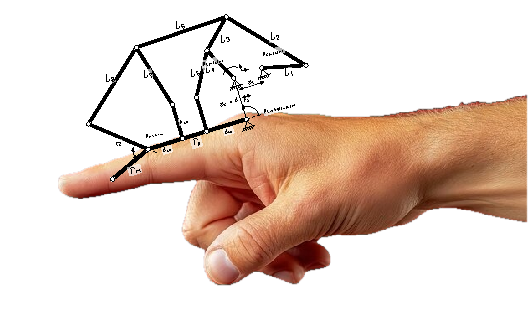
\includegraphics[width=\linewidth]{mecanismo_sobre_dedo_sin_dos_angulos.pdf}};
\end{tikzpicture}
\endgroup

\caption{Mecanismo simplificado del exoesqueleto montado sobre un dedo. Se conserva la geometría del diseño base antes de optimizar. $\theta_{1\mathrm{inicial}}$ corresponde a $L_4$ y $\theta_{2\mathrm{inicial}}$ a $L_1$, respecto a la horizontal positiva.}
\label{fig:dedo}
\end{figure}

Las juntas de revoluta se dibujan como círculos y los apoyos fijos con achurado. El modelo se detiene en la falange medial; la etapa distal del mecanismo completo no forma parte de esta comparación. Las longitudes del dedo índice utilizadas son $F_p=46$ mm y $F_m=27$ mm. La falange distal mide 22 mm, pero no interviene en el estudio parcial.

La base mantiene fijos MCF y los dos pivotes de entrada. Se emplean $B_1=18$ mm, $B_2=20$ mm y una relación de transmisión $r_g=2$. Dada la orientación $\theta_2$ de $L_1$, la de $L_4$ se obtiene mediante
\begin{equation}
\theta_1=\theta_2/r_g+\theta_{off}.
\end{equation}
El desfase $\theta_{off}$ fija su posición relativa inicial. La cinemática directa resuelve sucesivamente las intersecciones de circunferencias impuestas por las longitudes de las barras, manteniendo la misma configuración de ensamble durante el recorrido. Así se obtienen las posiciones de IFP e IFD.

\section{Formulación del problema de optimización}
\subsection{Variables de diseño}
El vector de diseño contiene $L_1$--$L_8$, $c_2$, $h_{sp}$, $d_{sp}$, $\theta_{aux}$, la orientación inicial y el recorrido de $L_1$, el desfase $\theta_{off}$ y una rotación fija del mecanismo respecto a la referencia. Se mantienen constantes las bancadas, las falanges y la relación 2:1. La Tabla~\ref{tab:limites} resume los límites empleados. El ángulo auxiliar describe la geometría del cuerpo medial y no es, por sí solo, un límite de flexión de la articulación.

\begin{table}[t]
\caption{Variables de diseño y límites de búsqueda}
\label{tab:limites}\centering\footnotesize
\begin{tabular}{lrr}\toprule Parámetro & Mín. & Máx.\\\midrule
$L_1$ (mm)&29.147&45.147\\ $L_2$ (mm)&31.205&51.205\\
$L_3$ (mm)&12.187&28.187\\ $L_4$ (mm)&14.633&28.633\\
$L_5$ (mm)&9.906&21.906\\ $L_6$ (mm)&51.273&71.273\\
$L_7$ (mm)&18.805&34.805\\ $L_8$ (mm)&38.985&58.985\\
$c_2$ (mm)&29.349&45.349\\ $h_{sp}$ (mm)&18.974&28.974\\
$d_{sp}$ (mm)&4.663&12.663\\ $\theta_{aux}$ (rad)&0.596&1.196\\
Ángulo inicial de $L_1$ (rad)&$-0.545$&0.155\\
Desfase $\theta_{off}$ (rad)&1.378&2.078\\
Recorrido de $L_1$ (rad)&1.663&2.663\\
Rotación de montaje (rad)&2.661&3.361\\\bottomrule
\end{tabular}
\end{table}

\subsection{Función objetivo}
La base de datos pública de Jarque-Bou, Atzori y Müller \cite{r1} contiene registros cinemáticos de distintos movimientos y agarres de la mano. Para este estudio se dispone de un archivo de 120 muestras angulares, correspondientes a un agarre fino. Sus ángulos se convierten en posiciones usando las longitudes de las falanges indicadas. Para la búsqueda se seleccionan 32 muestras distribuidas a lo largo del recorrido; los errores de trayectoria se calculan después sobre las 120 muestras.

El ajuste considera las diferencias entre los ángulos articulares del mecanismo y de la referencia. Cada diferencia se multiplica por la longitud de la falange correspondiente y se combina con penalizaciones por falta de cierre, separación insuficiente del dedo, posición fuera del dorso, altura excesiva y transmisión desfavorable. Si $r_j$ es cada componente de ese conjunto de errores y penalizaciones, se minimiza
\begin{equation}
J=\frac{1}{N_r}\sum_{j=1}^{N_r}r_j^2.
\label{eq:objetivo}
\end{equation}
Los componentes se expresan en mm mediante sus factores de ponderación, por lo que $J$ se expresa en mm$^2$. Este valor sirve para dirigir la búsqueda; no es el error de posición de las trayectorias.

Los factores empleados son 1 para el error angular multiplicado por la longitud, 30 para cierre, 4 para separación, posición dorsal y altura, y 0.5 mm/grado para transmisión. Las penalizaciones se activan al superar el límite correspondiente. Se conserva el mismo objetivo para ED y AG. La sensibilidad a la ponderación angular se revisa en la discusión.

La Tabla~\ref{tab:restricciones} resume las condiciones que se comprueban al seleccionar las soluciones finales. Una penalización pequeña no sustituye esta revisión geométrica. Se evalúan 501 posiciones por solución y se repite la comprobación con 5001 posiciones para los diseños seleccionados.

\begin{table}[t]
\caption{Restricciones geométricas del modelo parcial}
\label{tab:restricciones}\centering\footnotesize
\begin{tabular}{p{.37\columnwidth}p{.52\columnwidth}}\toprule
Condición & Comprobación\\\midrule
Cierre de los cuatro lazos & Defecto máximo $\leq10^{-7}$ mm\\
Geometría del soporte & $F_p>2d_{sp}$; dimensiones positivas\\
Separación del dedo & Holgura estimada $\geq1$ mm\\
Ubicación dorsal & Distancia dorsal firmada $\geq1$ mm\\
Altura sobre el dedo & Estimación planar $<55$ mm\\
Transmisión & Ángulo mínimo $\geq25^\circ$\\\bottomrule
\end{tabular}
\end{table}

Para estimar separación y altura se revisan 17 puntos de cada barra. En el plano del movimiento se representa el dedo mediante una franja de 6 mm a cada lado de su eje y se reserva un margen de 3 mm para la barra. Son aproximaciones geométricas usadas por igual en ambas optimizaciones, no medidas del espesor del CAD. El ensamble actual emplea eslabones de 4 mm de espesor; las interferencias entre sólidos y tornillos deben comprobarse en el modelo tridimensional.

\section{Evaluación de las técnicas de optimización}
Ambos algoritmos se ejecutan con 20 semillas, de 0 a 19, y 4096 evaluaciones de la función objetivo por ejecución. Cada evaluación corresponde a probar un vector de diseño completo. Se usa una población de 64 individuos, incluidos en ese presupuesto. Para cada semilla se comparte la población inicial y un mismo diseño de partida; no se introduce la solución de la semilla 12 como punto inicial.

Los parámetros de variación seleccionados mediante Optuna \cite{r13} son el intervalo del factor de mutación y la probabilidad de recombinación de ED, y las probabilidades de cruza y mutación y sus índices de distribución para AG. En las ejecuciones comparadas se mantienen fijos en los valores indicados a continuación. No se utilizan ajuste local ni paro anticipado, para respetar el mismo presupuesto en ambos métodos. El código se ejecuta en Python con NumPy; SciPy se utiliza en el análisis estadístico. Las medias y desviaciones estándar se calculan sobre las 20 ejecuciones, incluidas aquellas cuya mejor solución no satisface todas las condiciones de la Tabla~\ref{tab:restricciones}.

\subsection{Evolución Diferencial}
La Evolución Diferencial es una técnica poblacional para optimización en espacios continuos, cuyas variantes y aplicaciones se describen en \cite{r14,r15}. Se implementa la estrategia \texttt{best1bin}: cada vector de prueba parte del mejor individuo y de la diferencia escalada entre otros dos. El factor de mutación $F$ se toma de una distribución uniforme entre 0.54 y 0.85, una vez por generación; controla cuánto influye esa diferencia. La probabilidad de recombinación $CR=0.77$ decide qué componentes del vector de prueba se heredan de la mutación, forzando al menos uno. La selección conserva el vector de prueba si su objetivo no empeora el del individuo sustituido. La población se actualiza una vez evaluados los candidatos de la generación.

El intervalo de $F$ controla los tamaños de cambio que se prueban y $CR$ regula la combinación de componentes nuevos con los del individuo que se modifica. Estos son parámetros del algoritmo, no dimensiones del mecanismo.

La mutación diferencial adapta el tamaño de los cambios a la dispersión de la población. Cuando los individuos están separados, los cambios pueden ser mayores; cuando se concentran, los cambios tienden a reducirse. Esto describe el operador, pero no garantiza que siempre encuentre la mejor solución.

\subsection{Algoritmo Genético}
Se implementa un AG real codificado con selección por torneo de tamaño 3, cruza binaria simulada (SBX) \cite{r16} y mutación polinomial. La probabilidad de cruza por pareja es 0.63, con selección de cada componente con probabilidad 0.5. La mutación se aplica por variable con probabilidad 0.22. Los índices de distribución son 16 para SBX y 14 para mutación. En las generaciones completas se conservan dos individuos de élite y se reutilizan sus evaluaciones. En la última se generan únicamente dos descendientes para completar el presupuesto y se conservan los otros 62 individuos.

El torneo favorece a los individuos de menor objetivo, la cruza combina valores de dos padres y la mutación introduce variaciones adicionales. Los índices de distribución controlan qué tan cerca suelen quedar los nuevos valores de los anteriores; los dos individuos de élite conservan las mejores soluciones. La probabilidad 0.5 por componente es una regla de la cruza, mientras que las probabilidades 0.63 y 0.22 y los índices 16 y 14 definen su configuración. La población tiene 64 individuos en ambos métodos.

\section{Resultados}
\subsection{Error de ajuste}
La Tabla~\ref{tab:resultados} reúne los resultados de ambos métodos y los errores de sus soluciones seleccionadas. Se elige, para cada algoritmo, la ejecución de menor $J$ que cumple las restricciones: semilla 12 para ED y semilla 7 para AG. El error global de posición se calcula como la raíz del promedio de las distancias cuadráticas de los dos puntos IFP e IFD respecto al objetivo.

\begin{table}[t]
\caption{Comparación de ED y AG con presupuesto equivalente}
\label{tab:resultados}\centering\footnotesize
\begin{tabular}{lrr}\toprule Métrica & ED & AG\\\midrule
Ejecuciones &20&20\\ Evaluaciones por ejecución &4096&4096\\
Media de $J$ (mm$^2$)&0.001484&0.001504\\
Desviación estándar (mm$^2$)&0.001069&0.001192\\
Soluciones que cumplen restricciones&14/20&11/20\\\midrule
Semilla seleccionada&12&7\\
$J$ seleccionado (mm$^2$)&0.000419&0.000242\\
Error global RMSE (mm)&0.2976&0.1976\\
RMSE IFP (mm)&0.2162&0.1693\\
RMSE IFD (mm)&0.3611&0.2223\\
Altura estimada máxima (mm)&51.016&54.376\\\bottomrule
\end{tabular}
\end{table}

El AG obtiene el menor error global y el menor error en los dos puntos para estas soluciones. Por otro lado, la ED presenta una media de $J$ ligeramente menor y más soluciones que cumplen las restricciones. Se aplica la prueba de rangos con signo de Wilcoxon \cite{rwilcoxon}, que compara las diferencias entre pares sin exigir normalidad; su interpretación supone simetría en la distribución de esas diferencias. Cada par corresponde a una misma semilla y población inicial. La prueba bilateral sobre las 20 diferencias de $J$ no detecta una diferencia significativa ($W=105$, $p=1.000$, nivel 0.05). Esto no demuestra equivalencia ni una superioridad general de un algoritmo.

\begin{figure*}[t]
\centering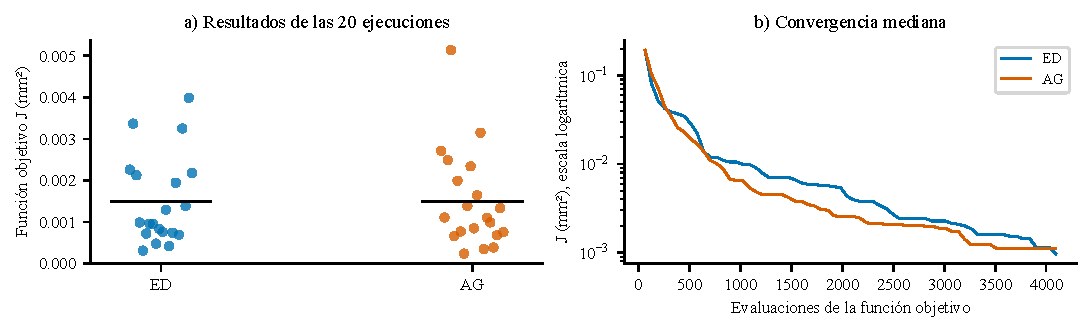
\includegraphics[width=\textwidth]{comparacion_semilla12.pdf}
\caption{Comparación entre ED y AG: (a) cada punto representa el mejor objetivo de una ejecución y la línea negra indica la media; (b) convergencia mediana de las 20 ejecuciones frente al número de evaluaciones.}
\label{fig:convergencia}
\end{figure*}

\subsection{Análisis dimensional}
La Tabla~\ref{tab:dimensiones} compara, eslabón por eslabón, las dimensiones del diseño CAD base frente a las optimizadas por ED y AG. La suma de $B_1$, $B_2$, $L_1$--$L_8$ y $c_2$ es de 328.29 mm para ED, 353.36 mm para AG y 380.01 mm para el diseño base. La solución ED tiene una suma 7.09\% menor que AG y una altura planar estimada de 51.02 mm, frente a 54.38 mm. Esto favorece su elección cuando se busca reducir el tamaño sobre la mano.

La compacidad es deseable para la fabricación y la portabilidad del dispositivo. Sin embargo, la suma de longitudes no equivale al peso ni al volumen del ensamble. Una reducción de masa dependerá también de las secciones, materiales, soportes y elementos de unión.

\begin{table}[t]
\caption{Dimensiones de los eslabones (mm): diseño CAD base y soluciones seleccionadas de ED y AG}
\label{tab:dimensiones}\centering\footnotesize\begin{tabular}{lrrr}\toprule Parámetro & CAD base & ED & AG\\\midrule
$B_1$ & 18.00 & 18.00 & 18.00\\
$B_2$ & 20.00 & 20.00 & 20.00\\
$L_1$ & 35.00 & 30.33 & 39.56\\
$L_2$ & 49.00 & 40.17 & 42.40\\
$L_3$ & 25.00 & 21.01 & 27.52\\
$L_4$ & 20.00 & 16.55 & 15.57\\
$L_5$ & 25.00 & 13.72 & 14.82\\
$L_6$ & 55.00 & 55.99 & 64.25\\
$L_7$ & 35.00 & 29.13 & 31.49\\
$L_8$ & 52.00 & 46.90 & 40.74\\
$c_2$ & 46.01 & 36.50 & 39.02\\
$h_{sp}$ & 17.00 & 23.71 & 21.83\\
$d_{sp}$ & 18.00 & 7.28 & 7.62\\
\midrule $\sum L_{est}$ & 380.01 & 328.29 & 353.36\\\bottomrule\end{tabular}
\end{table}

\subsection{Seguimiento de las trayectorias}
La Fig.~\ref{fig:trayectorias} muestra las trayectorias calculadas por ED y AG junto con la referencia angular utilizada. Ambas reproducen la forma general del movimiento. Los errores globales son 0.298 y 0.198 mm, respectivamente. La diferencia de ajuste favorece al AG, mientras que el tamaño de la solución favorece a ED.

El seguimiento se evalúa en posiciones correspondientes del recorrido, sin una alineación libre que reduzca el error. La distancia de Chamfer \cite{r11} y el ajuste de Procrustes \cite{r12} permiten estudiar semejanza de formas, pero no son las métricas empleadas en esta comparación. Aquí se conserva la relación entre la entrada de la manivela y el movimiento de las falanges.

\begin{figure*}[t]
\centering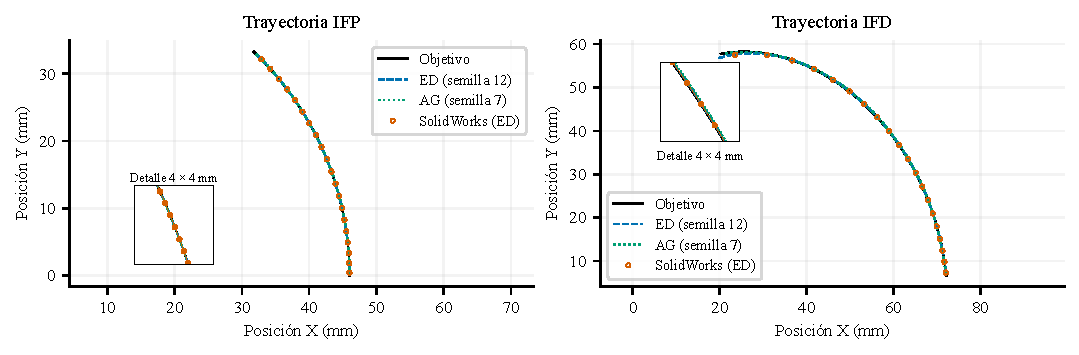
\includegraphics[width=\textwidth]{trayectorias_semilla12.pdf}
\caption{Trayectorias objetivo, de ED y de AG, y rutas de SolidWorks del diseño ED de la semilla 12. Los detalles de $4\times4$ mm muestran las diferencias sin desplazar las curvas.}
\label{fig:trayectorias}
\end{figure*}

\subsection{Convergencia}
La Fig.~\ref{fig:convergencia} muestra la disminución del objetivo durante la búsqueda. El eje horizontal representa evaluaciones, no generaciones, para comparar el mismo esfuerzo de cálculo. Se observa dispersión entre ejecuciones de ambos métodos. El presupuesto permite obtener soluciones útiles, pero no demuestra que se haya encontrado el mínimo global.

\subsection{Simulación del mecanismo optimizado}
Se construye el ensamble de la semilla 12 en SolidWorks con las falanges de 46 y 27 mm (Fig.~\ref{fig:cad}). Se exportan 60 posiciones del extremo de $L_1$, de IFP y de IFD en los mismos instantes. El ángulo de entrada se obtiene a partir del extremo de $L_1$ y su pivote fijo; se evalúa el modelo cinemático en esas mismas posiciones de entrada.

El estudio recorre 141.000$^\circ$, frente a los 139.295$^\circ$ de la solución optimizada. Se mantienen las 60 muestras para comparar SolidWorks con el modelo. La última queda fuera del intervalo de la referencia y no se utiliza en la comparación con el objetivo, que contiene 59 posiciones comunes.

\begin{figure}[t]
\centering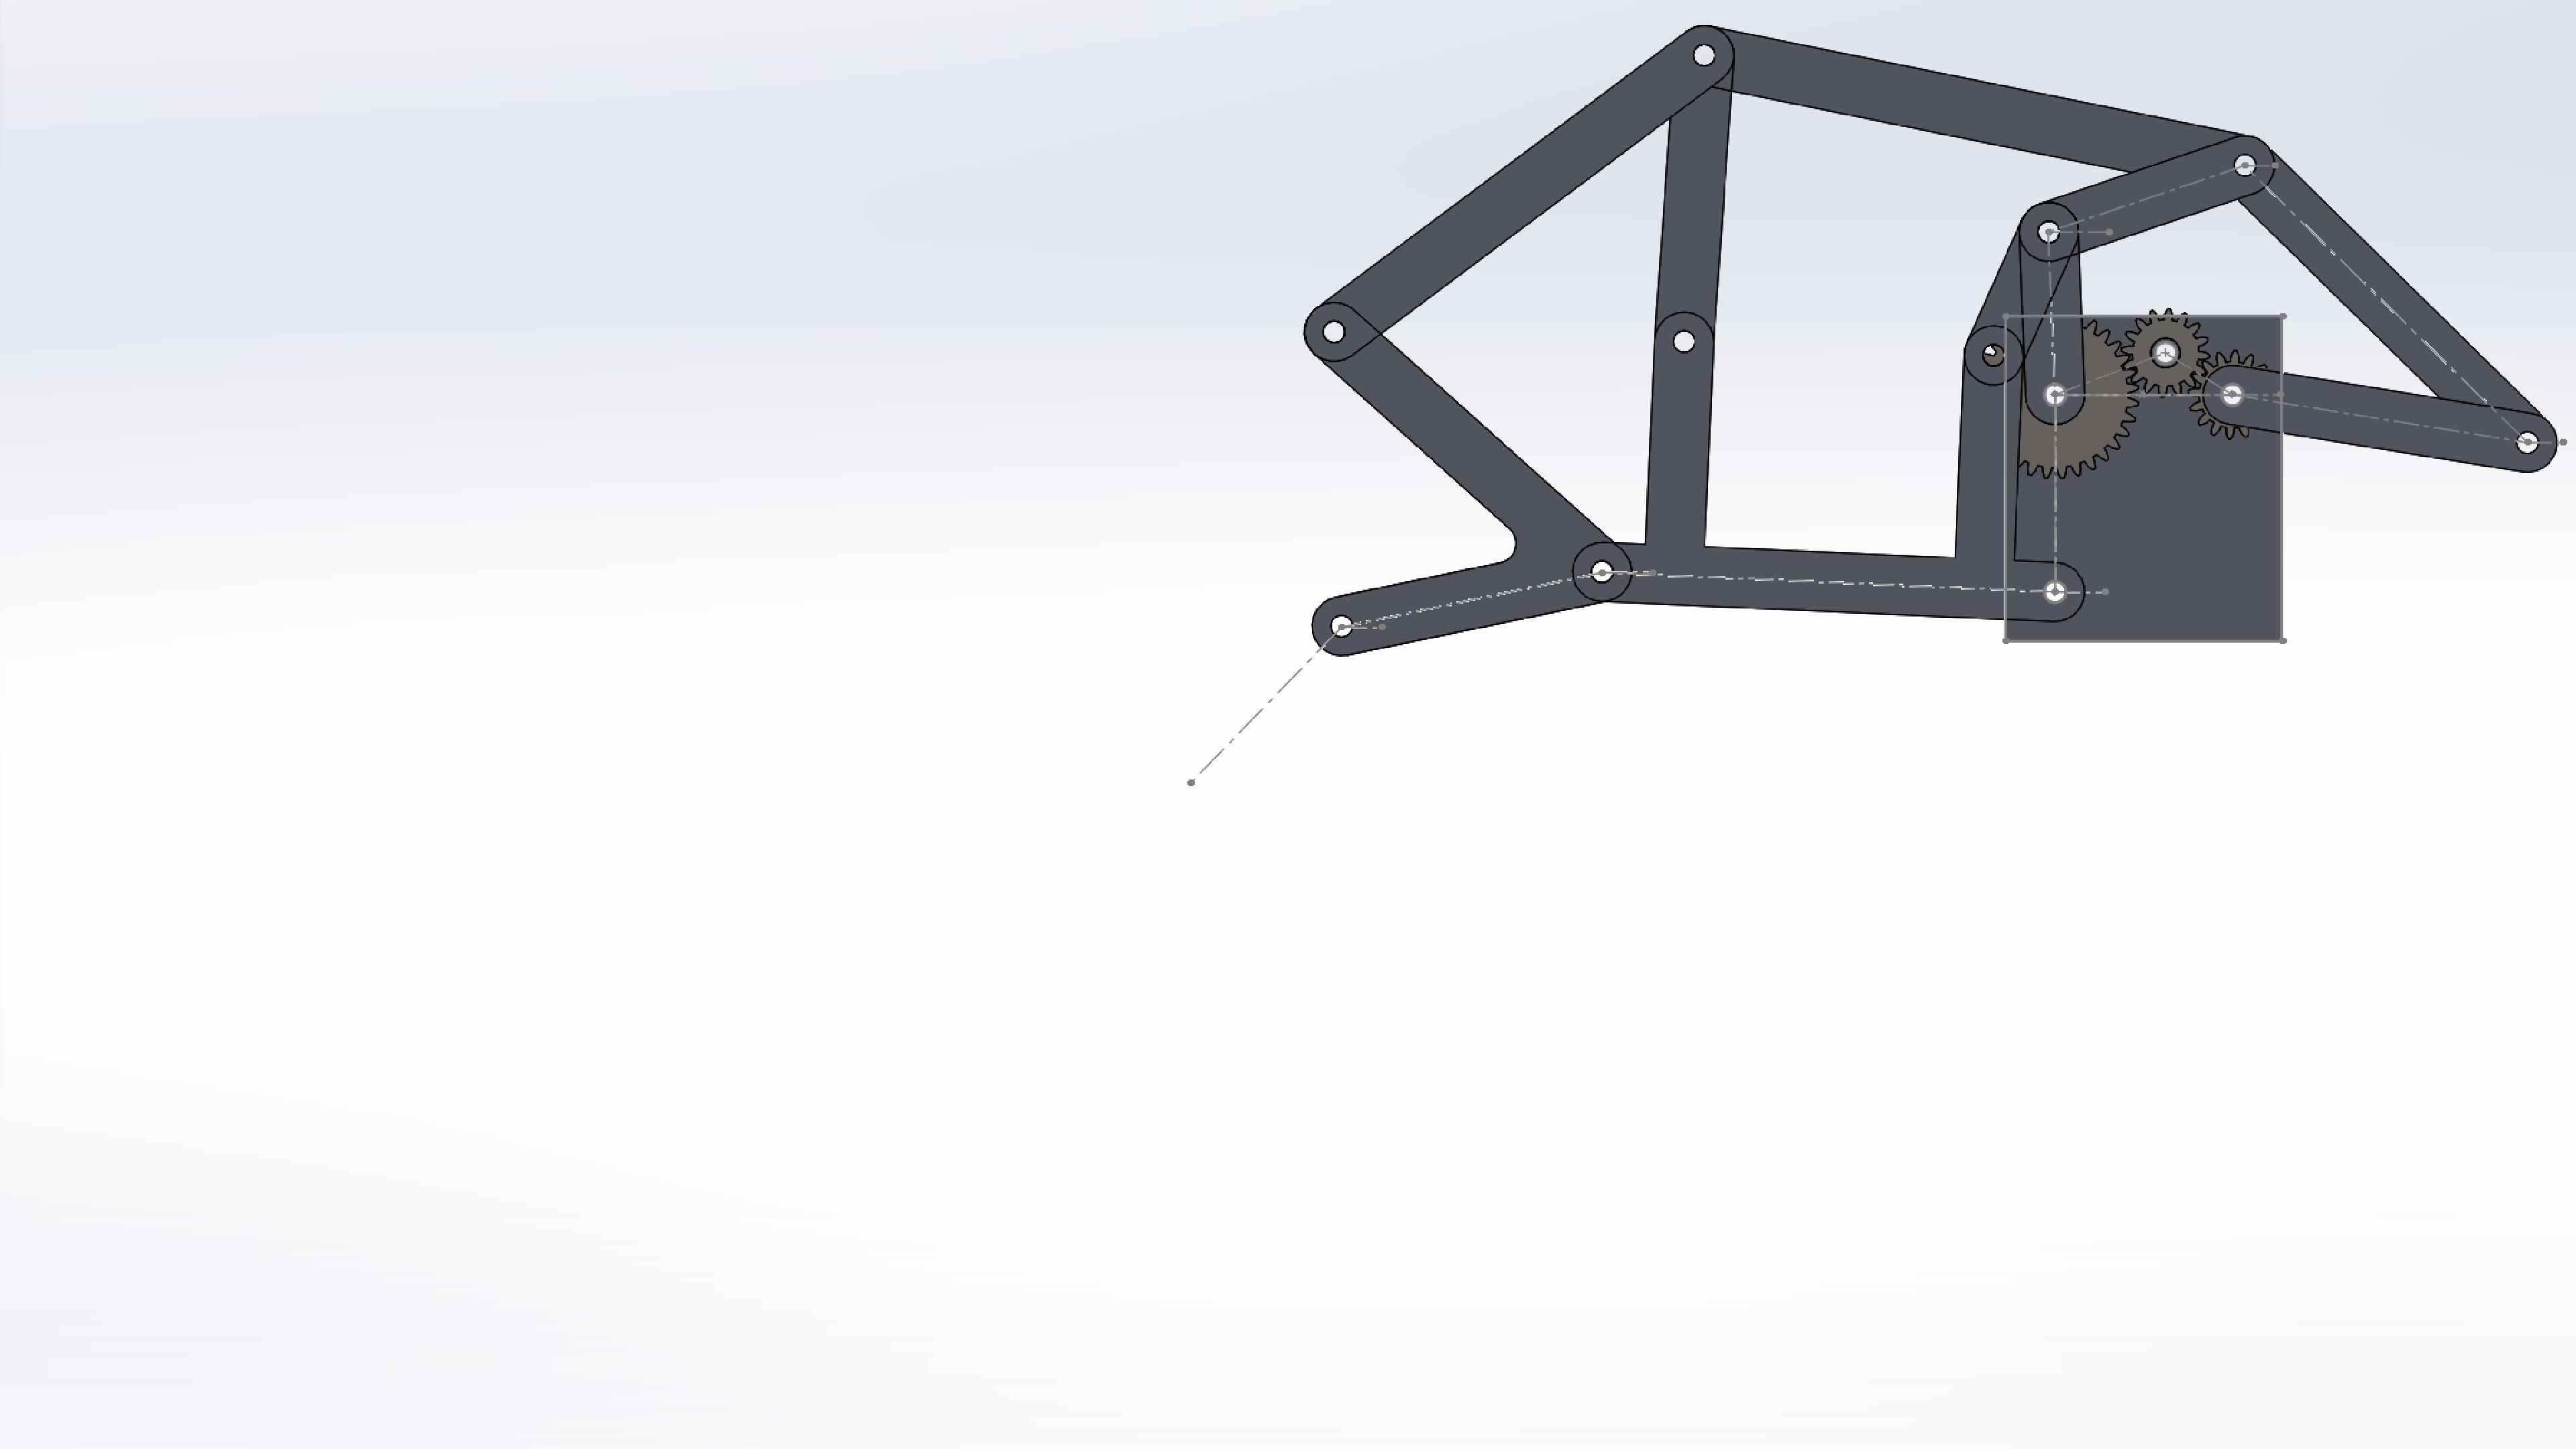
\includegraphics[width=\columnwidth,trim=330bp 195bp 0bp 0bp,clip]{CAD_semilla12.png}
\caption{Modelo CAD del mecanismo optimizado con ED, semilla 12, utilizado en el estudio de movimiento.}
\label{fig:cad}
\end{figure}

El error entre dos trayectorias correspondientes se calcula mediante
\begin{equation}
\mathrm{RMSE}=\sqrt{\frac{1}{N}\sum_{i=1}^{N}\|\mathbf p_i^{(1)}-\mathbf p_i^{(2)}\|^2}.
\end{equation}
La Tabla~\ref{tab:simulacion} distingue el error CAD--modelo del error respecto al objetivo. Las diferencias máximas CAD--modelo son 0.1150 mm en IFP y 0.2214 mm en IFD. Esta comparación comprueba que el ensamble reproduce la cinemática calculada; no constituye una medición de un prototipo físico.

\begin{table}[t]
\caption{RMSE de posición del mecanismo ED de la semilla 12}
\label{tab:simulacion}\centering\footnotesize
\begin{tabular}{lrr}\toprule Comparación & IFP (mm) & IFD (mm)\\\midrule
SolidWorks--modelo (60)&0.1065&0.1124\\
SolidWorks--objetivo (59)&0.2448&0.3884\\
Modelo--objetivo (59)&0.2178&0.3618\\\bottomrule
\end{tabular}
\end{table}

\section{Discusión}
El mecanismo seleccionado mantiene el ensamble durante el recorrido simulado. La ED construye cada nueva solución a partir de diferencias entre individuos; el AG real combina selección, cruza SBX y mutación polinomial. Ambos métodos encuentran mecanismos que siguen la referencia, aunque sus soluciones no son idénticas.

Para esta aplicación, la elección depende de la prioridad del diseño. Si se busca el menor error de trayectoria entre las soluciones seleccionadas, el AG ofrece el mejor resultado. Si se busca una menor suma de longitudes y menor altura calculada sobre el dedo, ED resulta preferible. Por esta razón se lleva a CAD la solución ED, sin descartar al AG como alternativa. El menor tamaño puede ayudar a reducir el volumen sobre la mano, pero el peso y la comodidad deben comprobarse con el diseño físico.

Para revisar la influencia de los pesos, se recalcula $J$ de los mismos diseños multiplicando los residuos angulares por 0.5, 1 y 2, sin cambiar las penalizaciones. Como los residuos se elevan al cuadrado, su aporte a $J$ se multiplica por 0.25, 1 y 4. Las medias ED/AG son, respectivamente, 0.000496/0.000543, 0.001484/0.001504 y 0.005437/0.005352 mm$^2$. El orden cambia en el último caso: la comparación depende de cuánto se valore el seguimiento angular. No se repite la optimización ni se modifican dimensiones o trayectorias.

El estudio se limita a la referencia angular disponible y a las medidas indicadas. La falta de identificación del registro original impide confirmar que el movimiento corresponda a una pinza fina; los resultados demuestran seguimiento de esa referencia y correspondencia CAD--modelo, no una validación del tipo de agarre. La simulación tampoco evalúa cargas, holguras de fabricación ni interferencias entre sólidos. Estas comprobaciones son necesarias antes de usar el mecanismo sobre una persona.

\section{Conclusión}
Se obtiene la síntesis dimensional parcial de un mecanismo de exoesqueleto de dedo mediante ED y AG, bajo el mismo planteamiento, función objetivo y presupuesto de evaluaciones, con 20 semillas por método. El AG seleccionado obtiene menor error global de trayectoria: 0.198 mm frente a 0.298 mm de ED. La ED entrega una menor suma de longitudes: 328.29 mm frente a 353.36 mm, por lo que se elige para continuar el desarrollo de un mecanismo compacto.

El ensamble de la semilla 12 en SolidWorks reproduce las trayectorias del modelo con RMSE de 0.106 mm en IFP y 0.112 mm en IFD. Se confirma la correspondencia cinemática entre ambos. Como trabajo futuro se contempla extender el análisis al mecanismo completo de tres falanges y comprobar el movimiento mediante un prototipo y medición de trayectorias.

\ifdefined\versionciega
  \IEEEtriggeratref{2}
\else
  \newpage
\fi
\begin{thebibliography}{18}
\bibitem{r1} N. J. Jarque-Bou, M. Atzori, and H. Müller, ``A large calibrated database of hand movements and grasps kinematics,'' \emph{Scientific Data}, vol. 7, art. 12, 2020, doi: \doi{10.1038/s41597-019-0349-2}.
\bibitem{r2} K. Xia \emph{et al.}, ``Hand exoskeleton design and human--machine interaction strategies for rehabilitation,'' \emph{Bioengineering}, vol. 9, no. 11, art. 682, 2022, doi: 10.3390/bioengineering9110682.
\bibitem{r3} R. John Varghese, G. Mukherjee, and A. Deshpande, ``Designing physical human-robot interaction interfaces: A scalable method for simulation based design,'' \emph{Frontiers in Neurorobotics}, vol. 15, art. 727534, 2022, doi: \doi{10.3389/fnbot.2021.727534}.
\bibitem{r4} J. A. Cabrera, A. Simon, and M. Prado, ``Optimal synthesis of mechanisms with genetic algorithms,'' \emph{Mechanism and Machine Theory}, vol. 37, no. 10, pp. 1165--1177, 2002, doi: 10.1016/S0094-114X(02)00051-4.
\bibitem{r5} S. Sleesongsom and S. Bureerat, ``Four-bar linkage path generation through self-adaptive population size teaching-learning based optimization,'' \emph{Knowledge-Based Systems}, vol. 135, pp. 180--191, 2017, doi: \doi{10.1016/j.knosys.2017.08.012}.
\bibitem{r6} V. Kachitvichyanukul, ``Comparison of three evolutionary algorithms: GA, PSO, and DE,'' \emph{Industrial Engineering \& Management Systems}, vol. 11, no. 3, pp. 215--223, 2012, doi: 10.7232/iems.2012.11.3.215.
\bibitem{r7} T. Tušar and B. Filipič, ``Differential evolution versus genetic algorithms in multiobjective optimization,'' in \emph{Evolutionary Multi-Criterion Optimization}, LNCS 4403, 2007, pp. 257--271, doi: 10.1007/978-3-540-70928-2\_22.
\bibitem{r8} S. M. Varedi-Koulaei, M. Mohammadi, M. A. M. Mohammadi, and M. Bamdad, ``Optimal synthesis of the Stephenson-II linkage for finger exoskeleton using swarm-based optimization algorithms,'' \emph{Journal of Bionic Engineering}, vol. 20, no. 4, pp. 1569--1584, 2023, doi: \doi{10.1007/s42235-022-00327-5}.
\bibitem{r9} Bilal, M. Pant, H. Zaheer, L. Garcia-Hernandez, and A. Abraham, ``Differential evolution: A review of more than two decades of research,'' \emph{Engineering Applications of Artificial Intelligence}, vol. 90, art. 103479, 2020, doi: \doi{10.1016/j.engappai.2020.103479}.
\bibitem{r10} A. K. Qin, V. L. Huang, and P. N. Suganthan, ``Differential evolution algorithm with strategy adaptation for global numerical optimization,'' \emph{IEEE Trans. Evolutionary Computation}, vol. 13, no. 2, pp. 398--417, 2009, doi: \doi{10.1109/TEVC.2008.927706}.
\bibitem{r17} J. A. Caballero-Mora \emph{et al.}, ``UR3 collaborative robot inverse kinematics using metaheuristic optimization: A unified comparative and experimental evaluation,'' \emph{Applied System Innovation}, vol. 9, no. 7, art. 140, 2026, doi: 10.3390/asi9070140.
\bibitem{r13} T. Akiba, S. Sano, T. Yanase, T. Ohta, and M. Koyama, ``Optuna: A next-generation hyperparameter optimization framework,'' in \emph{Proc. ACM SIGKDD}, 2019, pp. 2623--2631, doi: \doi{10.1145/3292500.3330701}.
\bibitem{r14} S. Das, S. S. Mullick, and P. N. Suganthan, ``Recent advances in differential evolution -- An updated survey,'' \emph{Swarm and Evolutionary Computation}, vol. 27, pp. 1--30, 2016, doi: \doi{10.1016/j.swevo.2016.01.004}.
\bibitem{r15} S. Chakraborty, A. K. Saha, A. E. Ezugwu, J. O. Agushaka, R. A. Zitar, and L. Abualigah, ``Differential evolution and its applications in image processing problems: A comprehensive review,'' \emph{Archives of Computational Methods in Engineering}, vol. 30, no. 2, pp. 985--1040, 2023, doi: \doi{10.1007/s11831-022-09825-5}.
\bibitem{r16} K. Deb and R. B. Agrawal, ``Simulated binary crossover for continuous search space,'' \emph{Complex Systems}, vol. 9, no. 2, pp. 115--148, 1995.
\bibitem{rwilcoxon} F. Wilcoxon, ``Individual comparisons by ranking methods,'' \emph{Biometrics Bulletin}, vol. 1, no. 6, pp. 80--83, 1945, doi: \doi{10.2307/3001968}.
\bibitem{r11} H. G. Barrow, J. M. Tenenbaum, R. C. Bolles, and H. C. Wolf, ``Parametric correspondence and chamfer matching: Two new techniques for image matching,'' in \emph{Proc. IJCAI}, 1977, pp. 659--663.
\bibitem{r12} J. C. Gower, ``Generalized Procrustes analysis,'' \emph{Psychometrika}, vol. 40, no. 1, pp. 33--51, 1975, doi: \doi{10.1007/BF02291478}.
\end{thebibliography}

\end{document}
